% Copyright 2026 Sreeram Anil
% SPDX-License-Identifier: CC-BY-4.0
% =============================================================================
%  Moving-horizon estimation, iterated to convergence (MHE)
% =============================================================================
\chapter{Moving-horizon estimation (MHE)}
\label{ch:mhe}

\section*{At a glance}
\begin{tabular}{@{}l>{\raggedright\arraybackslash}p{0.76\textwidth}@{}}
Family & optimization (moving horizon) \\
Header & \texttt{include/estkit/optimization/mhe.hpp} \\
Registered name & \texttt{MHE} (converged); see Chapter~\ref{ch:mherti} for \texttt{MHE-RTI} \\
State dimension & $n_x = 4$ (cell model) --- generic in $n_x, n_u, n_y$; horizon $N = 20$ \\
Decision variables & $(N{+}1)n_x = 84$ \\
Cost per step & $\mathcal{O}(n_\text{it}\,N\,n_x^3)$, linear in $N$;
measured \SI{32}{\micro\second}, no heap \\
Memory & \SI{26.9}{\kilo\byte} fixed arrays (window, Jacobians, factorisation) \\
Primary references & \cite{rao2003mhe,rawlings2017mpc,robertson1996mhe,bertsekas1982projnewton} \\
\end{tabular}

\section{Motivation and aerospace/BMS relevance}
Every recursive filter in this report compresses the whole past into a mean and a covariance and
then throws the measurements away.  That compression is exact for a linear Gaussian system and an
approximation for everything else --- and the approximation is made \emph{once per sample, and
never revisited}.  If the linearisation at sample $k$ was poor, the EKF cannot go back; the error
it committed is baked into $\Pplus_k$ and propagates forever.  Nor can a recursive filter respect
an inequality: the state of charge is physically confined to $[0,1]$ and the hysteresis state to
$[-1,1]$, but a Kalman update is an unconstrained linear-Gaussian operation, and the best it can do
is clip the result afterwards --- which silently makes the covariance inconsistent with the
estimate.

Moving-horizon estimation \citep{robertson1996mhe,rao2003mhe} takes the opposite position: keep the
last $N{+}1$ measurements, and at every sample re-solve the maximum-a-posteriori problem over the
whole window, subject to the constraints.  Everything older is summarised by one quadratic
\emph{arrival cost}, which is what makes the problem finite.  The price is obvious --- an
optimisation problem per sample instead of a matrix update --- and the benefits are three:
re-linearisation of the whole window at every sample, exact handling of the box constraints, and
the ability to trade computation for accuracy by choosing $N$.

For an electric-aircraft battery the specific attraction is the \texttt{combined} failure case:
a mis-estimated initial SOC, a biased current sensor, and a cell that has lost capacity, all at
once.  This is not a contrived scenario --- it is what a pack looks like after a season in service
with an uncalibrated shunt --- and it is where the EKF of Chapter~\ref{ch:ekf} fails outright
(\SI{12.4}{\percent} steady-state SOC error, never converging).  MHE reaches \SI{0.69}{\percent} on
the same data.  Section~\ref{sec:mhe-results} explains why.

\section{Problem statement and assumptions}
Consider the discrete-time system
\begin{equation}\label{eq:mhe-sys}
\vx_{j+1} = f(\vx_j,\vu_j) + \vw_j,\qquad
\vy_j = h(\vx_j,\vu_j) + \vv_j,\qquad
\vw_j\sim\N{0}{\mQ_j},\ \vv_j\sim\N{0}{\mR_j},
\end{equation}
with $\vx_j\in\real^{n_x}$, $\vu_j\in\real^{n_u}$, $\vy_j\in\real^{n_y}$, and a feasible set
\begin{equation}\label{eq:mhe-box}
\mathbb{X} = \{\,\vx\in\real^{n_x} : \vx^{\mathrm{lo}}\le \vx\le \vx^{\mathrm{hi}}\,\}.
\end{equation}
Write the window at time $k$ with local node indices $j = 0,\dots,n$, node $j$ holding the absolute
instant $k-n+j$, where $n = \min(k,N)$ so that the window grows from a single node at $k=0$ to its
full length at $k=N$.

\begin{assumption}[Detectability]\label{as:mhe-det}
The pair $(f,h)$ is (incrementally) detectable, so that the full-information estimator is a stable
observer.
\end{assumption}
\begin{assumption}[Bounded arrival cost]\label{as:mhe-arr}
The arrival-cost approximation $Z_{k-N}(\cdot)$ used in place of the exact one satisfies
$Z_{k-N}(\vx)\le Z^\star_{k-N}(\vx) + c$ for a finite $c$ and is bounded below by a
$\mathcal{K}_\infty$ function of $\norm{\vx-\vx^\star}$.
\end{assumption}

Under \cref{as:mhe-det,as:mhe-arr}, \citet[Thm.~4]{rao2003mhe} prove that the constrained
moving-horizon estimator is an asymptotically stable observer, and that $N$ must be at least the
observability index.  For the cell model the observability index is $1$: $\soc$ is instantaneously
observable through $\ocv(\soc,T)$ wherever $\partial\ocv/\partial\soc\neq 0$, which on this NMC
chemistry holds everywhere in $[0.05,0.98]$.  The horizon is therefore a \emph{noise-averaging and
constraint-handling} choice, not a feasibility one --- a point worth making, because it is what
lets $N$ be as small as $20$.

\section{Derivation}

\subsection{The nonlinear program}
Eliminating the noises from \cref{eq:mhe-sys} and taking negative logarithms of the Gaussian
densities turns the maximum-a-posteriori problem over the window into
\begin{equation}\label{eq:mhe-nlp}
\boxed{
\begin{aligned}
\min_{\vx_0,\dots,\vx_n}\ \ \Phi \;=\;
&\tfrac12\norm{\vx_0 - \bar\vx}^2_{\Pi^{-1}}
\;+\;\tfrac12\sum_{j=0}^{n-1}\norm{\vw_j}^2_{\mQ_j^{-1}}
\;+\;\tfrac12\sum_{j=0}^{n}\norm{\vv_j}^2_{\mR_j^{-1}} \\
\text{s.t.}\quad
&\vw_j = \vx_{j+1} - f(\vx_j,\vu_j),\qquad j = 0,\dots,n-1, \\
&\vv_j = \vy_j - h(\vx_j,\vu_j),\qquad\ \ j = 0,\dots,n, \\
&\vx_j\in\mathbb{X},
\end{aligned}}
\end{equation}
with $\norm{a}^2_{\mW} = a^\T\mW a$.  Because the noises are eliminated rather than kept as
decision variables, the states are the only unknowns: this is the \emph{multiple-shooting}
parameterisation \citep{bock1984multipleshooting}, in which the dynamics appear as penalised
residuals instead of eliminated equalities.  Multiple shooting matters here for a numerical reason:
a single-shooting formulation would propagate $\vx_0$ through $N$ steps of $f$, so the sensitivity
of the last node to the first would be $\prod_j \mF_j$ --- badly conditioned as soon as the RC
branches decay --- whereas in \cref{eq:mhe-nlp} every node is an independent variable and the
Hessian stays banded and well scaled.

\subsection{Arrival cost}
The first term of \cref{eq:mhe-nlp} must summarise everything the data \emph{before} the window
said about $\vx_{k-n}$, i.e.\ the density $p(\vx_{k-n}\mid \vy_{0:k-n-1})$.  For a linear Gaussian
system this density is exactly Gaussian and \cref{eq:mhe-nlp} reproduces the Kalman filter; for a
nonlinear system it is not available in closed form, and \citet{rao2003mhe} propose the
\emph{filtering} approximation: propagate $\Pi$ by the EKF covariance recursion along the optimal
trajectory.  Concretely, when the window slides past the node holding instant $t$,
\begin{align}
\mS &= \mH_t\,\Pi\,\mH_t^\T + \mR_t, \label{eq:mhe-arrS}\\
\mK &= \mF_t\,\Pi\,\mH_t^\T\,\mS^{-1}, \label{eq:mhe-arrK}\\
\Pi^{+} &= \mQ_t + \mF_t\,\Pi\,\mF_t^\T - \mK\,\mS\,\mK^\T, \label{eq:mhe-arrP}\\
\bar\vx^{+} &= f(\hat\vx_t, \vu_t), \label{eq:mhe-arrx}
\end{align}
with $\mF_t = \partial f/\partial\vx$, $\mH_t = \partial h/\partial\vx$ evaluated at the leaving
node.  \Crefrange{eq:mhe-arrS}{eq:mhe-arrP} is the \emph{prior-to-prior} Riccati recursion: it takes
the prior at instant $t$, folds in the measurement $\vy_t$ (which is leaving the window) and
predicts one step, so $\Pi^{+}$ carries exactly the information in $\vy_{0:t}$ --- precisely what
the new window, which starts at $t+1$, must not count again.

The mean \cref{eq:mhe-arrx} admits two readings of $\hat\vx_t$, and the choice matters more than
any other tuning decision in this chapter \citep[Sec.~4.3.2]{rawlings2017mpc}:
\begin{description}[leftmargin=2.2em,style=nextline]
\item[Filtering update] $\hat\vx_t = \hat\vx_{t|t}$, the estimate of that node produced when it was
the \emph{newest} node of the window.  It summarises $\vy_{0:t}$ exactly once, so mean and
covariance are statistically consistent.
\item[Smoothing update] $\hat\vx_t = \hat\vx_{t|t+N}$, the node's \emph{current} value in the window
about to be discarded.  That value has been fitted to $\vy_{t+1:t+N}$, which the next window uses
again; those measurements are therefore counted twice while $\Pi$ is not shrunk accordingly.
\end{description}
Statistically the filtering update is the correct one, and on this benchmark it is measurably
better whenever the model is right and the data are noisy.  It is also measurably \emph{worse}
whenever the model is wrong, because a consistent arrival cost keeps shrinking and then refuses to
let the window explain a persistent modelling error.  \Cref{tab:mhe-arrival} gives the numbers;
the smoothing update is registered, and \cref{sec:mhe-impl} explains the reasoning.

\begin{table}[H]\centering
\caption{Effect of the arrival-mean convention. Steady-state SOC RMSE [\%] on the eVTOL mission,
\texttt{MHE-RTI}, $N = 20$, seed~1 (development run; the registered configuration's three-seed
values are in Table~\ref{tab:cell_MHERTI}).}
\label{tab:mhe-arrival}
\begin{tabular}{@{}lcccccc@{}}
\toprule
& \texttt{nominal} & \texttt{noise\_step} & \texttt{cold} & \texttt{dropout} & \texttt{aged} & \texttt{combined}\\
\midrule
EKF baseline        & 0.06 & 0.06 & 0.15 & 0.91 & 1.30 & 12.22 \\
Filtering update    & 0.08 & \textbf{0.13} & \textbf{0.19} & \textbf{0.11} & 7.08 & 4.84 \\
Smoothing update \emph{(registered)}
                    & 0.06 & 1.33 & 0.93 & 0.53 & \textbf{0.70} & \textbf{0.49} \\
Filtering, $\Pi\times3$ & 0.08 & 0.30 & 0.35 & 0.07 & 3.07 & 4.09 \\
\bottomrule
\end{tabular}
\end{table}

\subsection{Gauss--Newton and the KKT structure}
Write \cref{eq:mhe-nlp} as $\Phi = \tfrac12\norm{\bm{r}(\mathcal{X})}^2$ with the stacked variable
$\mathcal{X} = (\vx_0,\dots,\vx_n)\in\real^{(n+1)n_x}$ and the weighted residual stack $\bm{r}$.
Linearising $\bm{r}$ about the current iterate and dropping the second-derivative term gives the
Gauss--Newton normal equations \citep[\S10.3]{nocedal2006}
\begin{equation}\label{eq:mhe-normal}
\bm{M}\,\delta\mathcal{X} = -\bm{g},\qquad \bm{M} = \mathcal{J}^\T\mW\mathcal{J},\quad \bm{g} = \mathcal{J}^\T\mW\bm{r} .
\end{equation}
Because each residual touches at most two consecutive nodes, $\bm{M}$ is \emph{block tridiagonal}:
\begin{align}
\bm{M}_{jj} &= \underbrace{[j{=}0]\,\Pi^{-1}}_{\text{arrival}}
          + \underbrace{[j{>}0]\,\mQ_{j-1}^{-1}}_{\text{from } \vw_{j-1}}
          + \underbrace{[j{<}n]\,\mF_j^\T\mQ_j^{-1}\mF_j}_{\text{from } \vw_j}
          + \underbrace{\mH_j^\T\mR_j^{-1}\mH_j}_{\text{from } \vv_j}, \label{eq:mhe-A}\\
\bm{M}_{j,j+1} &= -\mF_j^\T\mQ_j^{-1} \;=:\; \mB_j, \qquad \bm{M}_{j+1,j} = \mB_j^\T,
\label{eq:mhe-B}\\
\bm{g}_j &= [j{=}0]\,\Pi^{-1}(\vx_0-\bar\vx) + [j{>}0]\,\mQ_{j-1}^{-1}\vw_{j-1}
        - [j{<}n]\,\mF_j^\T\mQ_j^{-1}\vw_j - \mH_j^\T\mR_j^{-1}\vv_j .
\label{eq:mhe-g}
\end{align}
This banded structure is the whole point: the KKT system of a moving-horizon problem is never
dense, and exploiting it is what makes MHE affordable \citep{wangboyd2010fastmpc}.

\subsection{Block-tridiagonal factorisation}
$\bm{M}$ is factored by a block $\mL\mD\mL^\T$ sweep \citep[\S4.3]{golubvanloan2013}, never assembled
as an $(n{+}1)n_x$ square matrix:
\begin{equation}\label{eq:mhe-ldl}
\begin{aligned}
&\mD_0 = \bm{M}_{00}, &&\vz_0 = -\bm{g}_0, \\
&\mL_j = \mB_{j-1}^\T\mD_{j-1}^{-1}, \quad
 \mD_j = \bm{M}_{jj} - \mL_j\mB_{j-1}, &&\vz_j = -\bm{g}_j - \mL_j\vz_{j-1},
 \qquad j = 1,\dots,n, \\
&\delta\vx_n = \mD_n^{-1}\vz_n, \quad
 \delta\vx_j = \mD_j^{-1}\bigl(\vz_j - \mB_j\,\delta\vx_{j+1}\bigr), && j = n-1,\dots,0 .
\end{aligned}
\end{equation}
Correctness follows from $\mL_j\mD_{j-1}\mL_j^\T = \mB_{j-1}^\T\mD_{j-1}^{-1}\mB_{j-1} = \mL_j\mB_{j-1}$,
so that $(\mL\mD\mL^\T)_{jj} = \bm{M}_{jj}$ and $(\mL\mD\mL^\T)_{j,j-1} = \mB_{j-1}^\T$ as required.
The recursion is the information-form dual of the Riccati sweep of a linear-quadratic regulator;
its cost is $\mathcal{O}\bigl((n{+}1)n_x^3\bigr)$, i.e.\ \emph{linear} in the horizon, against
$\mathcal{O}\bigl((n{+}1)^3 n_x^3\bigr)$ for a dense solve --- a factor of $441$ at $N = 20$ and
$2601$ at $N = 50$.

\begin{proposition}[Marginal covariance]\label{prop:mhe-marg}
After the forward sweep of \cref{eq:mhe-ldl}, $\mD_n$ is the Schur complement of $\bm{M}$ onto the last
block, hence $\mD_n^{-1} = (\bm{M}^{-1})_{nn}$ is the Gauss--Newton (Laplace) posterior covariance of
the current state estimate.
\end{proposition}
\begin{proof}[Proof sketch]
The forward sweep eliminates blocks $0,\dots,n-1$ in order; block elimination of a symmetric matrix
leaves the Schur complement onto the remaining block, and for a Gaussian (quadratic) objective the
inverse of the Schur complement of the information matrix is the marginal covariance.
\end{proof}
\Cref{prop:mhe-marg} is what lets an MHE report a covariance at all; \texttt{P()} returns
$\mD_n^{-1}$ and the benchmark's $\pm2\sigma$ band is drawn from it at no extra cost.

\subsection{Constraints: projected Gauss--Newton}
The box \cref{eq:mhe-box} is enforced by a \emph{projected} step \citep{bertsekas1982projnewton}:
the unconstrained direction is computed from \cref{eq:mhe-ldl} and the iterate is then clipped,
\begin{equation}\label{eq:mhe-proj}
\vx_j \leftarrow \mathcal{P}_{\mathbb{X}}\bigl(\vx_j + \alpha\,\delta\vx_j\bigr),
\qquad
\bigl[\mathcal{P}_{\mathbb{X}}(\vx)\bigr]_i = \min\bigl(\max(x_i, x^{\mathrm{lo}}_i), x^{\mathrm{hi}}_i\bigr).
\end{equation}
This is \emph{exact} whenever the solution is interior --- the projection is then inactive and
\cref{eq:mhe-proj} is an ordinary Newton step --- and returns a feasible, generally suboptimal point
otherwise.  It is a gradient/Newton-projection step, not an active-set QP solve: for a separable
box and a positive-definite Hessian, projection preserves descent along each coordinate, but the
Newton direction is not recomputed on the active face, so a solution sliding along a constraint is
approached rather than attained.  That trade is deliberate.  On the cell problem the constraints
$\soc\in[0,1]$, $h\in[-1,1]$ are inactive for almost the whole mission and matter only during large
transients --- a \SI{35}{\percent} initial SOC error, a stuck voltage sensor, a hysteresis state
driven past saturation --- which is exactly where feasibility is what one wants and optimality is
irrelevant.  Retaining feasibility also keeps $\ocv(\soc)$ inside its tabulated range, which is a
real robustness benefit: an unconstrained iterate that wanders to $\soc = -0.3$ would be evaluated
on the linear extrapolation of the OCV table and could produce an arbitrary Jacobian.

The iteration terminates on the relative step norm
\begin{equation}\label{eq:mhe-tol}
\max_{j,i}\ \frac{|\delta x_{j,i}|}{1+|x_{j,i}|} \;<\; \texttt{tol} = \num{e-5},
\end{equation}
or after \texttt{max\_iter} $= 5$ iterations, whichever comes first.  An optional cost-decrease
safeguard (halve $\alpha$ until $\Phi$ decreases, up to \texttt{backtrack\_max} times) is available
and disabled by default; see \cref{sec:mhe-impl}.

\section{Algorithm}
\begin{algorithm}[H]
\caption{MHE --- one sampling period}
\begin{algorithmic}[1]
\Require window $\{\vx_j,\vu_j,\vy_j\}_{j=0}^{n}$, arrival $(\bar\vx,\Pi)$, new $\vu_{k-1}$, $\vy_k$, $\vu_k$
\Statex \textbf{Slide and warm start} (\texttt{predict})
\If{$n < N$} \State $n\gets n+1$;\ \ $\vx_n \gets f(\vx_{n-1},\vu_{k-1})$
\Else
  \State advance the arrival cost past node $0$ by \crefrange{eq:mhe-arrS}{eq:mhe-arrx}
  \State shift $\vx_j\!\gets\!\vx_{j+1},\ \vu_j\!\gets\!\vu_{j+1},\ \vy_j\!\gets\!\vy_{j+1}$ for $j<N$
  \State $\vx_N \gets f(\vx_{N-1},\vu_{k-1})$ \Comment{shift-and-append warm start}
\EndIf
\Statex \textbf{Solve} (\texttt{update}, with $\vy_n\gets\vy_k$, $\vu_n\gets\vu_k$)
\State $\mQ_j^{-1}\gets \bigl[\mQ(\vx_j,\vu_j)\bigr]^{-1}$, $\mR_j^{-1}\gets\bigl[\mR(\vx_j,\vu_j)\bigr]^{-1}$, $\Pi^{-1}$
       \Comment{frozen at the entry iterate}
\For{$\text{it} = 1,\dots,\texttt{max\_iter}$}
  \State evaluate $\mF_j,\mH_j,\vw_j,\vv_j$ at all nodes;\ \ assemble $\bm{M}_{jj},\mB_j,\bm{g}_j$ by
         \crefrange{eq:mhe-A}{eq:mhe-g}
  \State factor and solve by the block $\mL\mD\mL^\T$ sweep \cref{eq:mhe-ldl}
  \State $\vx_j \gets \mathcal{P}_{\mathbb{X}}(\vx_j + \alpha\,\delta\vx_j)$ for all $j$ \Comment{\cref{eq:mhe-proj}}
  \State \textbf{break} if the step norm satisfies \cref{eq:mhe-tol}
\EndFor
\Ensure $\hat\vx_k = \vx_n$, $\mP_k = \mD_n^{-1}$ (\cref{prop:mhe-marg})
\end{algorithmic}
\end{algorithm}

\section{Application to the battery model}
For the ECM of Chapter~\ref{ch:ecm}, $n_x = 4$, $n_u = 2$, $n_y = 1$, $\dt = \SI{0.1}{\second}$ and
$N = 20$, so the window spans \SI{2}{\second} and holds $84$ decision variables and $21$ voltage
measurements.  The box is $\soc\in[0,1]$ and $h\in[-1,1]$; the RC voltages are left free, since they
are bounded by the current but not by any known constant.  $\mQ$ and $\mR$ come from the model
unchanged (the current-sensor noise mapped through $\mB$, plus the diagonal floors), so MHE and EKF
solve the same statistical problem and any difference between them is attributable to the horizon,
the constraints or the arrival cost --- not to tuning.

Two implementation choices deserve naming.  First, $\mQ_j^{-1}$, $\mR_j^{-1}$ and $\Pi^{-1}$ are
computed \emph{once} per sample at the entry iterate and held fixed through the Gauss--Newton loop:
they depend on the state only through the process-noise mapping, and re-evaluating them inside the
loop would change the objective being minimised from one iteration to the next.  Second, the
arrival-cost update \crefrange{eq:mhe-arrS}{eq:mhe-arrP} is performed \emph{before} the window is
shifted, because it needs the leaving node's state, input and measurement.

\section{Implementation notes}
\label{sec:mhe-impl}
\paragraph{Why the smoothing update is registered.}  \Cref{tab:mhe-arrival} shows the statistically
consistent filtering update winning by factors of $3$--$10$ on \texttt{noise\_step}, \texttt{cold}
and \texttt{sensor\_dropout}, and losing by a factor of $10$ on \texttt{aged\_cell}.  The mechanism
is clear: with a consistent arrival cost, $\Pi$ converges to the steady-state prior covariance
($\Pi_{\soc\soc}\approx\num{9e-7}$, i.e.\ $\sigma_{\soc}\approx\SI{0.09}{\percent}$), which is an entirely
correct statement about a \emph{correct} model and a wildly overconfident one about a cell that has
silently lost \SI{15}{\percent} of its capacity, where the true state drifts away from the model at
$\approx\num{7e-6}$ per sample.  The smoothing update's double counting acts as an unintentional
fading memory: the arrival mean is continuously refreshed by the newest data, the effective memory
is shorter, and the estimator retains the agility to follow the drift.  Since \emph{every}
flight-representative scenario in this benchmark carries some model error, the smoothing update is
registered.  A deployment on a well-identified, well-instrumented cell should prefer
\texttt{ArrivalFiltered}, and the last row of \cref{tab:mhe-arrival} shows the principled middle
ground: the consistent update with $\Pi$ inflated by a constant factor, i.e.\ an explicit
fading-memory arrival cost in the sense of \citet{sorenson1971fading}.

\paragraph{Conditioning.}  The normal equations are genuinely ill-conditioned:
$\mQ^{-1}_{\soc\soc} = \num{e10}$ (the SOC process-noise floor is $\num{e-5}$ per step) while the
measurement contribution $\mH^\T\mR^{-1}\mH$ is $\mathcal{O}(\num{e5})$ and $\Pi^{-1}$ is
$\mathcal{O}(\num{e6})$, so $\kappa(\bm{M})\sim\num{e5}$ per block and the subtraction
$\mD_j = \bm{M}_{jj} - \mL_j\mB_{j-1}$ cancels two quantities of order $\num{e10}$ to leave one of
order $\num{e6}$.  Four to five decimal digits are lost, which double precision absorbs and
\texttt{float} does not, in principle.  In practice the \texttt{float} build reproduces the
double-precision results on every scenario of Table~\ref{tab:float} (\texttt{nominal} $0.10$ vs.\
$0.10$, \texttt{init\_error} $0.08$ vs.\ $0.10$, \texttt{aged\_cell} $0.81$ vs.\ $0.81$,
\texttt{combined} $0.59$ vs.\ $0.68$ --- the single-precision build is in fact slightly
\emph{better} on the last two), because the cancellation is structured (the two terms share the
factor $\mQ^{-1}$) rather than random.  A relative Levenberg term
$\mD_j \leftarrow \mD_j + \texttt{reg}\,(1+\norm{\mD_j}_\infty)\mI$ with $\texttt{reg} = \num{e-9}$
guards definiteness; every block inverse uses \texttt{solve\_spd} (Cholesky with an LU fallback) and
the sweep aborts, leaving the warm-started iterate untouched, if any factor becomes non-finite.
A square-root (QR) formulation of \cref{eq:mhe-ldl} would halve the condition number and is the
natural next step for a genuine single-precision target.

\paragraph{Memory and heap.}  Everything is a fixed-size array sized by $N$ and $n_x$: the window
($\vx,\vu,\vy$ and a backtracking copy), the cached $\mQ^{-1},\mR^{-1}$, the Jacobians
$\mF_j,\mH_j$, the residuals, and the four matrices $\bm{M}_{jj},\mB_j,\mD_j^{-1},\mL_j$ per node.
That is \SI{26.9}{\kilo\byte} at $N=20$ and \SI{63}{\kilo\byte} at $N=50$ in double
precision, all of it statically sized: no allocation, no recursion, and a worst-case
execution time bounded by the iteration cap times the per-iteration cost.

\paragraph{Backtracking.}  The cost-decrease safeguard is implemented (\texttt{backtrack\_max}) and
disabled by default.  Measured on seed~1 with two halvings allowed it changed \texttt{combined}
from \SI{0.44}{} to \SI{1.16}{\percent} and \texttt{noise\_step} from \SI{1.46}{} to
\SI{2.24}{\percent}: on a filtering problem the
objective \cref{eq:mhe-nlp} is a local model of the posterior, and insisting that \emph{it} decrease
at every iteration is not the same as improving the estimate.  Pure Gauss--Newton was never
observed to diverge on this problem, which is consistent with the mild nonlinearity (only
$\ocv(\soc)$ is nonlinear in the state).

\paragraph{Timing.}  \SI{32}{\micro\second} per sample at $N=20$ with up to $5$ iterations,
against \SI{17}{\micro\second} for the single-iteration variant of Chapter~\ref{ch:mherti} and
\SI{0.48}{\micro\second} for the EKF.  The iteration counter shows $3$--$5$ iterations in transients
and $3$ in steady state; \cref{eq:mhe-tol} rarely triggers early, because the process-noise
weighting makes the relative step norm of the RC states small but not tiny.  On a Cortex-M7 at
\SI{400}{\mega\hertz} the same code would take roughly \SI{1.4}{\milli\second} --- affordable at
\SI{10}{\hertz} for a single cell, and the reason a pack-level implementation would run MHE on a
representative cell and EKFs on the rest.  At $67\times$ the EKF it is the most expensive estimator
of either of these two families.

\section{Benchmark results}
\label{sec:mhe-results}
% Copyright 2026 Sreeram Anil
% SPDX-License-Identifier: CC-BY-4.0
\begin{table}[H]\centering\footnotesize\setlength{\tabcolsep}{4pt}
\caption{MHE: cell-level benchmark on the eVTOL mission (mean over seeds; RMSE and max error in \% SOC; $t_\mathrm{conv}$: first time the error stays below 2\,\% for 60\,s, -- = never; EKF reference: steady-state RMSE of the plain EKF on the same data).}\label{tab:cell_MHE}
\begin{tabular}{llrrrrrcrr}\toprule
plant & scenario & RMSE & RMSE$_\mathrm{ss}$ & max & $t_\mathrm{conv}$ [s] & RMSE$_v$ [mV] & div. & EKF ref. & ns/step \\ \midrule
ECM & nominal & 0.33 & 0.11 & 1.42 & 0 & 0.85 & no & 0.05 & 32403 \\
ECM & init\_error & 0.20 & 0.10 & 1.03 & 0 & 2.14 & no & 0.05 & 32450 \\
ECM & current\_bias & 0.54 & 0.09 & 2.07 & 0 & 0.88 & no & 0.61 & 32105 \\
ECM & noise\_step & 0.79 & 0.98 & 2.26 & 0 & 3.75 & no & 0.12 & 36396 \\
ECM & outliers & 1.44 & 0.49 & 4.33 & 340 & 2.62 & no & 0.21 & 34325 \\
ECM & cold & 0.82 & 0.77 & 2.69 & 0 & 1.93 & no & 0.16 & 32937 \\
ECM & hot & 0.26 & 0.04 & 1.24 & 0 & 0.62 & no & 0.03 & 32061 \\
ECM & aged\_cell & 1.29 & 0.79 & 5.79 & 0 & 3.41 & no & 1.52 & 32618 \\
ECM & param\_mismatch & 2.06 & 1.98 & 5.27 & 0 & 2.72 & no & 1.36 & 32022 \\
ECM & sensor\_dropout & 1.48 & 0.41 & 6.70 & 0 & 2.00 & no & 0.46 & 32207 \\
ECM & preisach & 0.87 & 0.46 & 3.22 & 156 & 0.86 & no & 0.20 & 32211 \\
ECM & combined & 0.79 & 0.69 & 4.44 & 0 & 4.40 & no & 12.44 & 32731 \\
\midrule
SPM & nominal & 3.31 & 3.45 & 3.94 & 0 & 1.02 & no & 3.73 & 28644 \\
SPM & init\_error & 4.12 & 4.25 & 4.97 & 0 & 2.17 & no & 3.81 & 28739 \\
SPM & current\_bias & 5.10 & 5.88 & 6.90 & 0 & 1.09 & no & 5.69 & 28464 \\
SPM & noise\_step & 4.78 & 5.95 & 9.41 & 0 & 3.78 & no & 3.30 & 29699 \\
SPM & outliers & 2.20 & 2.57 & 4.20 & 82 & 2.67 & no & 1.99 & 29091 \\
SPM & cold & 5.77 & 5.63 & 7.32 & 25 & 4.41 & no & 7.35 & 28479 \\
SPM & hot & 2.82 & 2.99 & 3.32 & 0 & 0.71 & no & 2.16 & 28715 \\
SPM & param\_mismatch & 5.11 & 5.73 & 7.01 & 0 & 1.86 & no & 3.13 & 29175 \\
SPM & sensor\_dropout & 5.66 & 5.88 & 6.54 & 0 & 2.10 & no & 5.31 & 28570 \\
\bottomrule\end{tabular}\end{table}

\begin{figure}[H]\centering
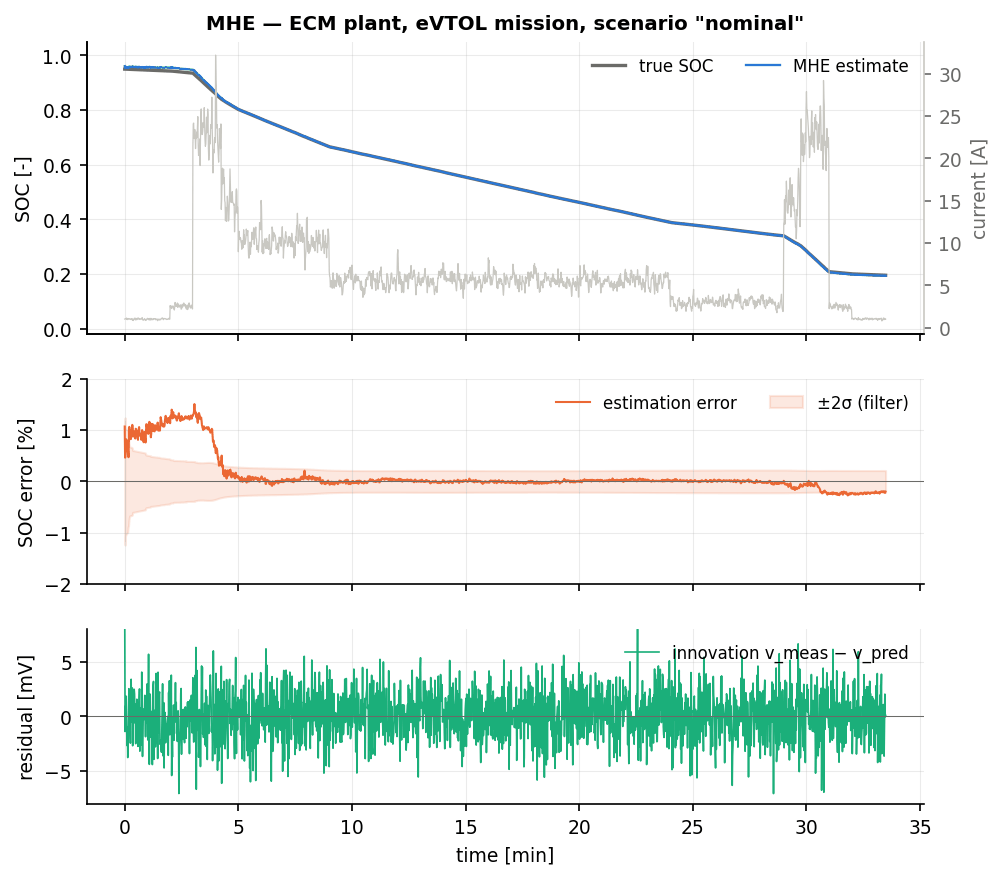
\includegraphics[width=\textwidth]{figures/cell_MHE_nominal.png}
\caption{MHE on the nominal eVTOL mission: true and estimated SOC (top), estimation error with the
$\pm2\sigma$ band from $\mD_n^{-1}$ (\cref{prop:mhe-marg}) (middle), voltage residual (bottom).}
\end{figure}
\begin{figure}[H]\centering
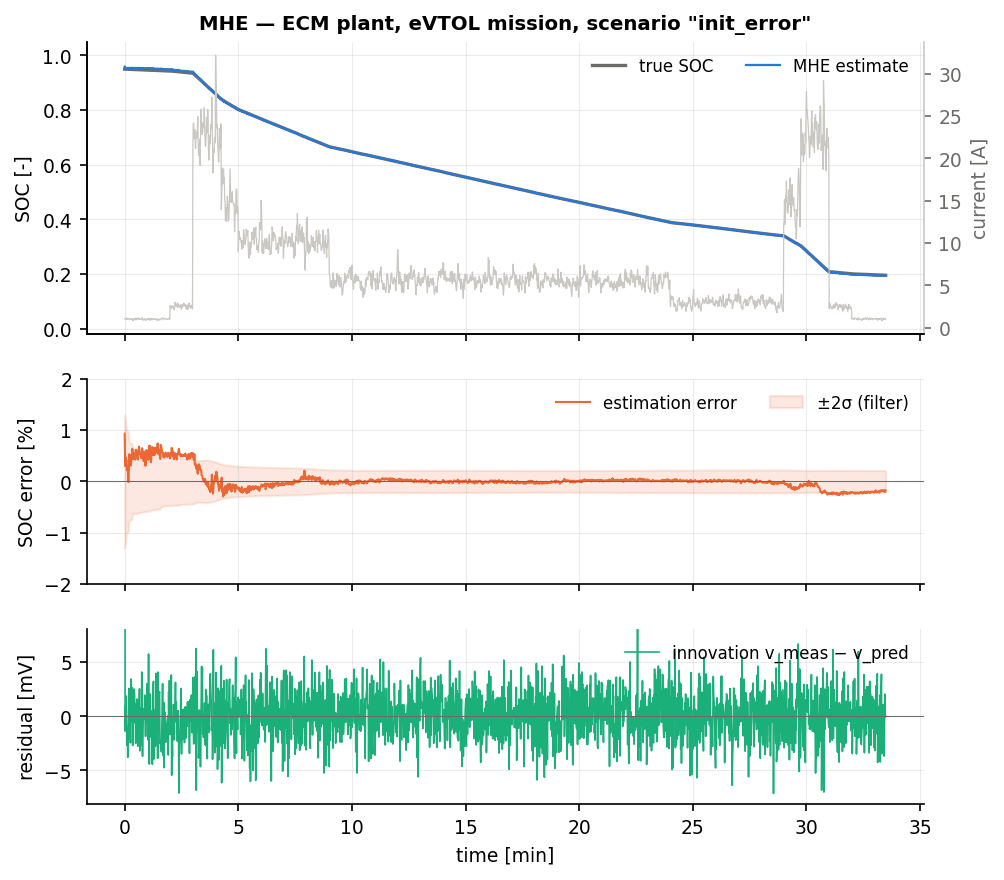
\includegraphics[width=\textwidth]{figures/cell_MHE_init_error.png}
\caption{MHE with a \SI{35}{\percent} initial SOC error.  The window is re-linearised at every
sample and the box $\soc\in[0,1]$ is enforced at every node, so the transient is removed within the
first sample and the covariance stays consistent with the constrained estimate.}
\end{figure}

All numbers below are three-seed means in per cent SOC from Table~\ref{tab:cell_MHE}.

\paragraph{Nominal and initial error.}  $\mathrm{rmse}/\mathrm{rmse_{ss}} =
0.33/\SI{0.11}{\percent}$ on \texttt{nominal} and $0.20/\SI{0.10}{\percent}$ on
\texttt{init\_error}, with $t_\text{conv} = \SI{0}{\second}$.  The EKF's steady-state error is
\SI{0.05}{\percent}, so the horizon costs a factor of two here.  That is the correct and
reassuring sign: with a well-matched model and an exact arrival cost, MHE and the Kalman filter
solve the same problem, and the residual difference is the arrival-cost approximation of
\cref{sec:mhe-impl} plus the two seconds at the start of the run during which the window is still
growing and the estimate is the maximum-a-posteriori solution of a very short record.  Both
estimators report the same voltage residual, $\mathrm{RMSE}_v = \SI{0.85}{\milli\volt}$ against the
EKF's \SI{0.79}{\milli\volt}: the model fits the data equally well in both, and what differs is
only how the past is summarised.

\paragraph{The headline result: \texttt{combined}.}  $0.79/\SI{0.69}{\percent}$ against the EKF's
$16.02/\SI{12.44}{\percent}$ --- a factor of \textbf{18} in steady-state error, and the difference
between an estimator that converges ($t_\text{conv} = \SI{0}{\second}$) and one that never does.
\texttt{combined} superposes a \SI{25}{\percent} initial SOC error, a \SI{0.15}{\ampere}
current-sensor bias with a \SI{2}{\percent} gain error, and \SI{10}{\percent} capacity loss.  The
EKF's covariance collapses during the benign opening minutes, after which its gain is too small to
fight the accumulating Coulomb-counting drift and it simply rides the bias down.  MHE resists for
two reasons that compound: the $21$-sample window is re-fitted from scratch at every step, so the
estimate is never the result of a gain the filter chose several hundred seconds ago; and the
arrival cost is re-anchored at every slide to a mean that has itself been re-fitted, which (as
\cref{sec:mhe-impl} explains) acts as a fading memory.  The two MHE variants are the only
estimators in the learning and optimization families below \SI{1}{\percent} on this scenario; the
best of the others, NN-Direct, is at \SI{4.09}{\percent} and the EKF-derived hybrids are above
\SI{9}{\percent}.

\paragraph{Where the horizon helps.}  \texttt{current\_bias} $0.54/\SI{0.09}{\percent}$ (EKF
$0.54/\SI{0.61}{\percent}$, a factor of \textbf{7} in steady state and the best result of any
estimator in this report on that scenario); \texttt{aged\_cell} $1.29/0.79$ (EKF $1.18/1.52$, a
factor of $1.9$); \texttt{sensor\_dropout} $1.48/0.41$ (EKF $0.72/0.46$); \texttt{outliers}
$1.44/0.49$ (EKF $0.52/0.21$ --- worse, see below); \texttt{hot} $0.26/0.04$, matching the EKF.
The \texttt{current\_bias} and \texttt{aged\_cell} results share one mechanism: both inject an
error into the \emph{state} equation, whose signature accumulates over time, and a window that
re-fits twenty-one samples jointly separates an accumulating drift from a state error far better
than a single Kalman gain can.  The dropout case additionally exercises the constraint: during the
\SI{15}{\second} stuck-voltage fault the estimate would leave $[0,1]$ in an unconstrained
formulation, and the projection \cref{eq:mhe-proj} keeps every node feasible, which is why the
steady-state error after the fault is \SI{11}{\percent} below the EKF's even though the peak
excursion is \SI{6.7}{\percent}, three times larger.

\paragraph{Where the horizon hurts.}  \texttt{noise\_step} $0.79/\SI{0.98}{\percent}$ (EKF
$0.18/\SI{0.12}{\percent}$), \texttt{cold} $0.82/0.77$ (EKF $0.20/0.16$) and
\texttt{param\_mismatch} $2.06/1.98$ (EKF $1.28/1.36$).  All three are direct consequences of the
registered arrival-mean convention: double counting the window's measurements is exactly wrong when
those measurements are noisier than $\mR$ claims (\texttt{noise\_step} raises $\sigma_v$ from
\SI{2}{\milli\volt} to \SI{20}{\milli\volt} at $t = \SI{600}{\second}$ without telling the
estimator), and the consistent filtering update recovers most of the EKF's performance on all three
(\cref{tab:mhe-arrival}).  This is the honest cost of the trade made in \cref{sec:mhe-impl}, and it
is a \emph{configuration} choice, not a property of moving-horizon estimation.
\texttt{param\_mismatch} is the worst ECM row of the sweep and deserves naming as such: a
\SI{30}{\percent} error in $R_0$ is a model error, and re-solving a twenty-one-sample fit of the
wrong model twenty-one times more carefully does not make it right --- it merely lets the estimate
chase the resulting voltage offset.

\paragraph{Outliers.}  $1.44/\SI{0.49}{\percent}$ against the EKF's $0.52/\SI{0.21}{\percent}$, and
the only scenario where MHE needs $t_\text{conv} = \SI{340}{\second}$ to settle inside
\SI{2}{\percent}.  MHE is \emph{not} robust to outliers, and it was never going to be:
\cref{eq:mhe-nlp} is a weighted least-squares problem, and least squares has an unbounded influence
function.  Fitting $21$ measurements jointly spreads a single $\SI{50}{\milli\volt}$ outlier over
the window rather than absorbing it in one step --- which is why the converged variant
(\SI{0.49}{\percent}) does better than the single-iteration one (\SI{0.70}{\percent}) --- but
spreading is not rejecting.  The constraints do not help because they are inactive.  Obtaining
genuine outlier robustness within this framework means replacing the quadratic
$\norm{\vv_j}^2_{\mR^{-1}}$ by a Huber or a Student-$t$ negative log-likelihood, which keeps the
banded structure and changes only the weights in \cref{eq:mhe-A}; that is the natural extension of
this chapter and the subject of the robust-filtering family, whose Huber-EKF reaches
\SI{0.06}{\percent} here.

\paragraph{Electrochemical (SPM) plant.}
\begin{figure}[H]\centering
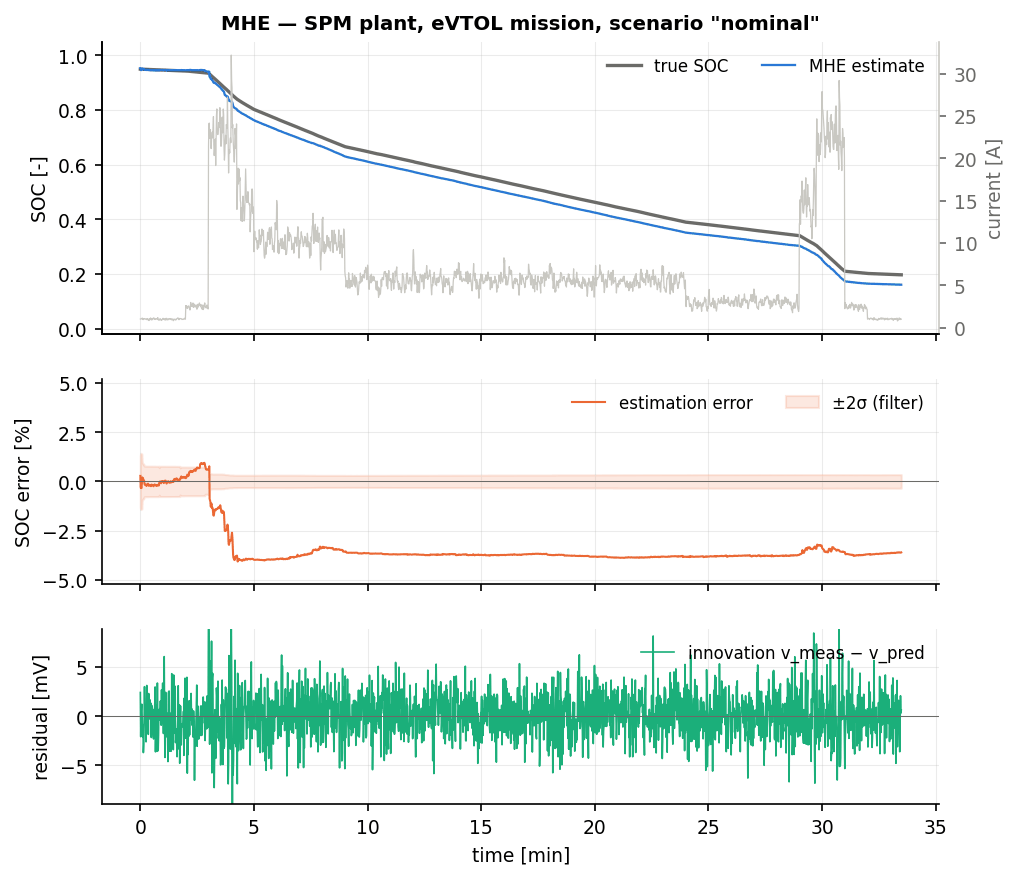
\includegraphics[width=\textwidth]{figures/cellspm_MHE_nominal.png}
\caption{MHE on the SPM plant, nominal eVTOL mission.  A two-second window cannot separate a
\SI{4}{\milli\volt} structured output residual from a state error, and the arrival cost is the only
mechanism that could discount it.}
\end{figure}
The SPM rows measure something the ECM rows cannot: robustness to \emph{structured} model error.
The truth plant is an electrochemical single-particle model with Butler--Volmer kinetics and slow
solid diffusion ($\tau_2 = \SI{556}{\second}$), and the estimators use a 2-RC ECM fitted to it,
which leaves a persistent \SI{4}{\milli\volt} residual in the output equation.  MHE gives
\SI{3.45}{\percent} on \texttt{nominal} against the EKF's \SI{3.73}{\percent}: a \SI{7}{\percent}
improvement, and the best of the two moving-horizon variants (MHE-RTI is at \SI{4.55}{\percent}),
but nowhere near the factor of eighteen it achieves on \texttt{combined}.  Across the nine SPM
scenarios it beats the EKF on only two --- \texttt{nominal} and \texttt{cold}
($\SI{5.63}{}$ vs.\ $\SI{7.35}{\percent}$, a \SI{23}{\percent} improvement) --- and loses on the
other seven, with \texttt{param\_mismatch} ($5.73$ vs.\ $3.13$), \texttt{noise\_step} ($5.95$ vs.\
$3.30$) and \texttt{hot} ($2.99$ vs.\ $2.16$) the worst.

The reason is structural and worth stating plainly, because it is the clearest limitation of the
whole approach.  \Cref{eq:mhe-nlp} assumes the model is right up to zero-mean process and
measurement noise.  A \SI{4}{\milli\volt} \emph{bias} in $h(\vx,\vu)$ violates that assumption in
the one place the formulation has no freedom: over a two-second window, twenty-one measurements all
carrying the same offset look exactly like a state that is displaced, and the least-squares fit
duly displaces it.  Re-linearising more carefully, iterating to convergence, or enforcing
$\soc\in[0,1]$ changes nothing --- all three make the estimator fit the wrong model \emph{better}.
The only element of the formulation that can help is the arrival cost, and only in its
inconsistent, smoothing form: because $\bar\vx$ is continuously refreshed from the newest window,
the estimator has a finite memory and the accumulated bias is partially discounted.  That is
precisely the mechanism that produces the modest \SI{7}{\percent} gain on \texttt{nominal} and the
\SI{23}{\percent} gain on \texttt{cold}, and its limits are visible in the field: the Fading-EKF,
which does nothing but discount old data explicitly and aggressively, reaches \SI{0.36}{\percent}
on the same row --- ten times better than MHE at a seventieth of the cost.  \textbf{A short horizon
with a wrong process model cannot beat a filter that simply stops believing its model.}  The
correct way to make MHE competitive here is not a longer horizon or more iterations but a larger
$\mQ$, an output-bias state appended to $\vx$, or the learned residual of
Chapter~\ref{ch:nnekf} inserted into $h$ --- all of which change the model rather than the
optimiser.  It is worth recording that the ECM results are unaffected by this: the excellent
\texttt{current\_bias} (\SI{0.09}{\percent}) and \texttt{combined} (\SI{0.69}{\percent}) figures
stand, because there the model \emph{is} the plant and the errors MHE is asked to resolve are
genuinely state-equation errors, which is exactly what a window is good for.

\paragraph{Horizon length.}  Measured with the registered configuration at $N\in\{10,20,50\}$
(steady-state RMSE [\si{\percent}], single Gauss--Newton iteration, seed~1):
\begin{center}
\begin{tabular}{@{}lccccccc@{}}
\toprule
$N$ & \texttt{nominal} & \texttt{outliers} & \texttt{noise\_step} & \texttt{param} & \texttt{aged} &
\texttt{combined} & \si{\micro\second}/step \\
\midrule
10 & 0.19 & 0.25 & 0.69 & 1.89 & 0.36 & 0.44 & \phantom{0}8.0 \\
20 & 0.06 & 0.90 & 1.33 & 2.25 & 0.70 & 0.49 & 14.2 \\
50 & 0.09 & 0.33 & 0.75 & 2.04 & 1.65 & 1.45 & 31.8 \\
\bottomrule
\end{tabular}
\end{center}
Cost grows linearly with $N$, as \cref{eq:mhe-ldl} promises, and accuracy does \emph{not} grow
monotonically.  Lengthening the window averages more measurements --- $N = 50$ is the best of the
three on \texttt{outliers} and \texttt{sensor\_dropout} --- but it also lengthens the lag between
the arrival cost and the present, which hurts precisely on the drifting scenarios
(\texttt{aged\_cell} degrades from $0.70$ to \SI{1.65}{\percent}).  For a system whose dominant
error is model drift rather than measurement noise, a short window is the better engineering
choice, and $N = 20$ (\SI{2}{\second}) sits at a reasonable compromise.  The general lesson is that
the horizon should be chosen against the \emph{ratio} of measurement noise to model error, not
maximised.

\section{Summary}
MHE re-solves a constrained maximum-a-posteriori problem over the last \SI{2}{\second} of data at
every sample, using multiple shooting, a filtering-based arrival cost, projected Gauss--Newton for
the box $\soc\in[0,1]$, $h\in[-1,1]$, and a block-tridiagonal $\mL\mD\mL^\T$ sweep whose cost is
linear in the horizon.  It is within a factor of two of the EKF where the EKF is right, it is the
best estimator in this report on \texttt{current\_bias} (\SI{0.09}{\percent} against
\SI{0.61}{\percent}), and it is one of only two that survive the \texttt{combined} scenario ---
\SI{0.69}{\percent} steady-state SOC error where the EKF has \SI{12.4}{\percent} and never
converges.  It costs \SI{32}{\micro\second} and \SI{27}{\kilo\byte}, roughly seventy times an EKF.
It is worse than the EKF wherever the measurement noise exceeds what $\mR$ declares --- a
consequence of the registered arrival-mean convention rather than of the method --- it has no
outlier robustness, and on the electrochemical plant, where the output equation carries a
structured \SI{4}{\milli\volt} bias, a two-second window cannot help and a plain fading-memory EKF
beats it tenfold.  Use it when model error lives in the \emph{state} equation and the constraints
are physically meaningful; use the real-time-iteration variant of Chapter~\ref{ch:mherti} when the
computation budget is tight, since it delivers most of the same benefit at half the cost.
